In this section, we introduce \emph{internal convergence}
(IntConv)
as a sound sufficient condition for ExtConv.
(In \secref{sec:detector}, we give an implementable detector for the IntConv criterion.)
Following the ``local-global'' structure of the problem, we will first define \emph{internal fixpoint} (IntFP) as a sound sufficient condition for an external fixpoint, and then
apply it
to all bracketed sub-circuits to 
formulate
the IntConv criterion.
At the end of this section, we give a qualitative data-dependency example in which relying on ExtConv without IntConv requires recursive trace-backs or additional retained state. The example provides a theoretical argument for an implementation benefit of IntConv.


Before introducing IntFP, we first introduce a natural generalization of \text{ZeroAfter} called \text{FixAfter}, which indicates that a stream becomes fixed to a constant value rather than to $0_A$.
\begin{definition}[FixAfter]
    Like \text{ZeroAfter}, \text{FixAfter} is a level-indexed predicate defined identically in its level-1, level-2, and vectorized forms, except that its base case $\text{FixAfter}_1(s, n)$ requires $\forall m \ge n,\, s[m] = s[n]$. Note that if $s$ is a nested stream $\stream{\stream{A}}$, this means repeating the exact same \emph{inner stream} $s[n]$ from the outer index $n$ onwards.
\end{definition}

Then, we reframe the FPD problem using a new level-indexed predicate called external fixpoint (ExtFP). Intuitively, ExtFP characterizes that a circuit reaches an external fixpoint at a given index, without looking into the internal circuit structure. Formally, 

\begin{definition}[External fixpoint (ExtFP)]
    Given any circuit $c$ (either level-1 or level-2), an input stream $x$, and an index $n \in \N$, we say that $c$ reaches an \emph{external fixpoint} across the first time dimension at $n$, denoted by $\text{ExtFP}_1(c, x, n)$, if both the input and the denoted output of $c$ are fixed after the outer index $n$:
    \[ \text{ExtFP}_1(c, x, n) := \text{FixAfter}_1(x, n) \land \text{FixAfter}_1(\means{c}(x), n) \]

    For a level-2 circuit $c$, a nested input stream $x \in \stream{\stream{A}}$, an outer index $m \in \N$, and an inner index $n \in \N$, the external fixpoint across the second time dimension is defined as:
    \[ \text{ExtFP}_2(c, x, m, n) := \text{FixAfter}_2(x, m, n) \land \text{FixAfter}_2(\means{c}(x), m, n) \]
    $\text{ExtFP}_2(c, x, \mathbf{b})$ for $\mathbf{b} \in \stream{\N}$ is naturally defined as $\forall i \in \N, \text{ExtFP}_2(c, x, i, \mathbf{b}[i])$.
\end{definition}

With this definition, the FPD problem for a level-1 circuit $c$ on input $x$ essentially asks to detect an index $n$ where $\text{ExtFP}_1(c, \delta_0(x), n)$ holds and the fixed output is $0$. Similarly, the FPD problem for a level-2 circuit $c$ on nested input $x$ asks to detect a bound stream $\mathbf{b}$ where $\text{ExtFP}_2(c, \lift{\delta_0}(x), \mathbf{b})$ holds and the fixed outputs are $0$.

As we proved in \secref{sec:fpd-undecidability}, exact FPD is impossible for sufficiently expressive circuits, and hence so is detecting ExtFP in full generality.
The Feldera implementation of DBSP~\cite{feldera_repo} uses internal-state stability to detect fixpoints. Each runtime operator provides a scope-indexed fixed-point check intended to report whether its output will remain stable if its input does, and the circuit combines the checks of its operators. Thus, the operational idea of detecting internal-state stability is established implementation practice rather than a novel contribution of this paper. The cited implementation specifies and tests this runtime contract, but does not provide a formal proof that the circuit-wide check implies denotational convergence.
To bridge the gap between this runtime strategy and the denotational DBSP theory, we give the strategy a rigorous, declarative account through a criterion called \emph{internal fixpoint} (IntFP). This formal criterion allows us to prove precisely this soundness connection, and later establish completeness for a large class of circuits. We discuss the relationship with the Feldera implementation further in \secref{sec:related}.

\begin{definition}[Internal fixpoint (IntFP)]\label{De:IntFP}
    Intuitively, IntFP means that all internal nodes (i.e., individual components) of a circuit have reached an ExtFP at a specific index.
    Formally, for any circuit $c$, an input stream $x$, and an index $n \in \N$, $\text{IntFP}_1(c, x, n)$ is defined by structural induction on $c$ over the categories in Table~\ref{tab:circuit-syntax}:
    \begin{itemize}
        \item \textbf{Primitive, Standard and Temporal Nodes:} Inherit the $\text{ExtFP}_1$ condition. That is, for any such node $c$, $\text{IntFP}_1(c, x, n) := \text{ExtFP}_1(c, x, n)$.
        \item \textbf{Structural Combinators:} Require $\text{IntFP}_1$ for all sub-circuits. That is
        \[\text{IntFP}_1(c_1 \seq c_2, x, n) := \text{IntFP}_1(c_1, x, n) \land \text{IntFP}_1(c_2, \means{c_1}(x), n)\] 
        and 
        \[\text{IntFP}_1(c_1 \pll c_2, x, n) := \text{IntFP}_1(c_1, x, n) \land \text{IntFP}_1(c_2, x, n)\].
        \item \textbf{Feedback Loops:} Require $\text{IntFP}_1$ for the loop body on the input tuple containing the delayed output. That is
        \[\text{IntFP}_1(\mathsf{loop}(c), x, n) := \text{IntFP}_1(c, (x, z^{-1}(\means{\mathsf{loop}(c)}(x))), n)\] 
        and similarly 
        \[\text{IntFP}_1(\mathsf{\lift{loop}}(c), x, n) := \text{IntFP}_1(c, (x, \lift{z^{-1}}(\means{\mathsf{\lift{loop}}(c)}(x))), n)\]
        \item \textbf{Level Adapters:} For $\mathsf{bracket}(c)$, $\text{IntFP}_1$ delegates to the level-2 internal circuit $c$: \[\text{IntFP}_1(\mathsf{bracket}(c), x, n) := \text{IntFP}_1(c, \lift{\delta_0}(x), n)\]
        For the level-1 circuit $\mathsf{lifting}(c)$, because it models an inner circuit that lacks states across outer iterations, the internal fixpoint naturally degenerates into the external fixpoint: 
        \[\text{IntFP}_1(\mathsf{lifting}(c), x, n) := \text{ExtFP}_1(\mathsf{lifting}(c), x, n)\]
    \end{itemize}
    The predicate $\text{IntFP}_2(c, x, m, n)$ for the second time dimension is defined for level-2 circuits only. It is mostly defined by uniformly replacing $\text{ExtFP}_1$ with $\text{ExtFP}_2$ and $\text{IntFP}_1$ with $\text{IntFP}_2$, with a notable exception. For the nested lifting circuit $\mathsf{lifting}(c)$, IntFP relies on the first dimension predicate $\text{IntFP}_1$ of the underlying level-1 circuit: 
    \[\text{IntFP}_2(\mathsf{lifting}(c), x, m, n) := \text{IntFP}_1(c, x[m], n)\]
    The vectorized version is naturally defined as $\text{IntFP}_2(c, x, \mathbf{b}) := \forall i \in \N, \text{IntFP}_2(c, x, i, \mathbf{b}[i])$.
\end{definition}

The definition of IntFP is both structural and level-indexed. For a bracketed circuit, it applies IntFP to the enclosed circuit, adapting the input to its stream level. Because the same rules apply recursively to sub-circuits, the definition also handles nested brackets.

One of the most important properties of IntFP is that it is a sound sufficient condition for $\text{ExtFP}$. That is, if a circuit reaches an internal fixpoint, it must have also reached an external fixpoint.

\begin{theorem}[Soundness of IntFP]\label{thm:intfp-sound}
    For any well-formed circuit $c$, input $x$, and index $n$, we have:
    \[ \text{IntFP}_1(c, x, n) \implies \text{ExtFP}_1(c, x, n) \]
    Similarly, for any level-2 circuit $c$, nested input $x$, and indices $m, n$:
    \[ \text{IntFP}_2(c, x, m, n) \implies \text{ExtFP}_2(c, x, m, n) \]
\end{theorem}
\begin{proof}
    We first prove the property for the level index 1, and then prove the property for the level 2 based on that for level 1. This can also be seen as induction on the level index of the predicate.
\end{proof}

Finally, by applying the local IntFP criterion to all bracketed sub-circuits, and adding that the fixed output is 0, we define our global convergence criterion called \emph{internal convergence} (IntConv).

\begin{definition}[Internal convergence (IntConv)]\label{def:intconv}
    We say that a circuit $c$ internally converges on input $x$, denoted $\text{IntConv}(c, x)$, if for any sub-circuit in the form of $\mathsf{bracket}(c_0)$ and its input $x_0$,
    \[\exists \mathbf{b},\, \text{IntFP}_2(c_0, \lift{\delta_0}(x_0), \mathbf{b}) \land \forall i, \means{c_0}(\lift{\delta_0}(x_0))[i][\mathbf{b}[i]] = 0\]
\end{definition}

By Theorem~\ref{thm:intfp-sound}, the definition of IntConv will be equivalent with $\forall i, \means{c_0}(\lift{\delta_0}(x_0))[i][\mathbf{b}[i]] = 0$ replaced by $\text{ZeroAfter}_2(\means{c_0}(\lift{\delta_0}(x_0)), \mathbf{b})$. This immediately implies that IntConv is a sound sufficient condition for ExtConv.
\begin{theorem}[Soundness of IntConv]\label{thm:intconv-sound}
    For any well-formed circuit $c$ and input $x$, we have
    \[\text{IntConv}(c, x) \implies \text{ExtConv}(c, x)\]
\end{theorem}

These soundness implications are one-way in general: ExtFP need not imply IntFP, and ExtConv need not imply IntConv. In \secref{sec:useful}, we identify circuit classes for which the corresponding converse does hold.

Why use IntConv rather than a weaker sound criterion for the theoretical specification ExtConv? The following example isolates one implementation benefit. For this circuit, an evaluator that relies only on ExtConv lacks a guarantee that earlier internal values have stabilized. It must therefore either recompute a recursive dependency chain or retain the historical values needed to answer later demands. IntConv supplies the missing stability guarantee.

Consider such a circuit satisfying ExtConv but not IntConv, with an integration operator $\mathcal{I}$ inside a bracketed sub-circuit, as shown in Fig.~\ref{fig:intconv-efficient}.
Its input $X$ and output $Y$ are both nested streams.
Assume ExtConv is detected soundly.
Suppose that evaluation is currently at $(4,3)$ (we use 1-based indexing)---namely, the third inner iteration of the fourth outer iteration---and that the first three outer iterations reached external convergence after two inner iterations, while the fourth did not.
Now $X[4][3]=12$ is ready.

\begin{figure}[!tb]
    \centering
    \begin{subfigure}[b]{0.48\textwidth}
        \centering
        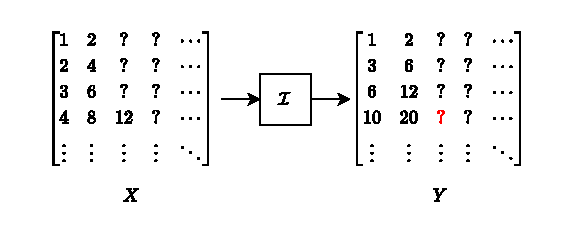
\includegraphics[width=\linewidth]{figures/intconv-efficient-1.pdf}
        \caption{An $\I$ operator inside a bracketed sub-circuit. The red \textcolor{red}{?} is the value we want to evaluate. }\label{fig:intconv-efficient-1}
    \end{subfigure}
    \hfill
    \begin{subfigure}[b]{0.48\textwidth}
        \centering
        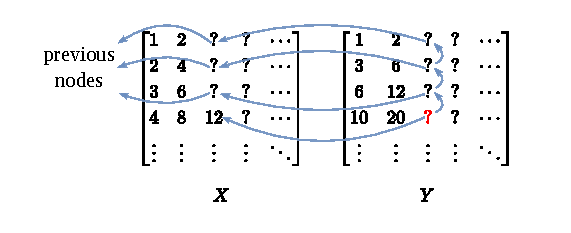
\includegraphics[width=\linewidth]{figures/intconv-efficient-2.pdf}
        \caption{Data dependency in this example. An arrow from $a$ to $b$ denotes that computing $a$ requires $b$.}\label{fig:intconv-efficient-2}
    \end{subfigure}
    \caption{A data-dependency cost that can arise when evaluation relies on ExtConv without IntConv.}\label{fig:intconv-efficient}
\end{figure}

Fig.~\ref{fig:intconv-efficient-2} shows the data dependency in this example. To evaluate $Y[4][3]$ correctly, we need
$Y[4][3] = Y[3][3] + X[4][3]$.
But because the circuit satisfies ExtConv without satisfying IntConv, external convergence does not guarantee internal convergence.
Consequently, we cannot directly conclude what $Y[3][3]$ is.
Computing $Y[3][3]$ may require $Y[2][3]$ and $X[3][3]$, both unknown; computing $X[3][3]$ can recursively force upstream re-evaluation, potentially all the way back to $\lift{\delta_0}$,
which initiated
the iterative computation.

Thus, under a strategy that does not retain all of this history, a later outer iteration that needs more inner iterations than earlier ones can trigger recursive recomputation. Retaining the history instead trades that recomputation for additional state, potentially across an unbounded number of outer iterations.

For this example, IntConv avoids that tradeoff.
Because IntConv guarantees that all internal nodes reach an internal fixpoint, values like $Y[3][3]$ are mathematically guaranteed to be stabilized values (e.g., $Y[3][3]=Y[3][2]$ in this example), which should already be stored in the state.
No recursive trace-back is needed, and state management stays simple: in this example, $\mathcal I$ only needs to store its output list (all output until convergence) from the last outer iteration.
This analysis is qualitative: it neither establishes a general lower bound for every criterion weaker than IntConv nor measures the overhead of a concrete implementation.
